\documentclass[11pt,a4paper]{ctexart}
\usepackage[margin=2.2cm]{geometry}
\usepackage{amsmath,amssymb}
\usepackage{graphicx}
\usepackage{booktabs,tabularx}
\usepackage{float}
\usepackage{caption}
\usepackage{hyperref}
\hypersetup{colorlinks=true,linkcolor=blue,urlcolor=blue}
\setlength{\parindent}{2em}
\setlength{\parskip}{0.3em}
\renewcommand{\arraystretch}{1.12}
\captionsetup{font=small}
\title{数据来源与获取说明}
\author{CQU\_MCM 2026 · 建模小组}
\date{2026-11-09}
\begin{document}
\maketitle
\thispagestyle{empty}
\newpage

\section*{摘  要}
本报告说明本项目所用数据的\textbf{全部来源、获取方式、处理链条与真实性边界}。气象与土壤水分来自 ECMWF \textbf{ERA5-Land} 再分析（经 Open-Meteo 历史天气接口获取），植被指数来自 NASA \textbf{MODIS MOD13Q1}（250 m、16 天合成 NDVI，经 ORNL DAAC 的 MODIS Web Service 取点）；两者都是公开、免注册的第三方科学数据，不是自造数据。共获得 8 个站点、960 个站-月记录（2015-01—2024-12），并据此派生植被覆盖度、输沙率与输沙势三个物理量；其中输沙率与输沙势由\textbf{真实风况}按已发表公式计算，仅保留一个整体标定系数，标定目标取自文献给出的年输沙率量级。

三条关键结论：① 数据链条完全可复现——脚本 01\_fetch\_real\_data.py 与 01b\_fetch\_ndvi.py 带缓存，重跑一次即可得到同样的面板；② 数据质量可验证——NDVI 的填充值（−3000）已识别，缺测率与云污染在报告中逐变量给出，并用 NASA POWER（MERRA-2）做了独立交叉验证；③ 数据边界清楚——\textbf{治理面积、投资、补水量不是观测数据}，它们是人工决策量，因此在数据集中单列为“情景参数”，不冒充观测值。


\section*{一、为什么选这套数据}
B 题三项任务需要六类输入：风况、降水、气温、土壤含水量、植被覆盖度、输沙率。赛题不提供数据，只能自行获取。判断一套数据能不能用的标准有三条：\textbf{空间上能落到防护带尺度}（几十米到几公里）、\textbf{时间上覆盖 10 年以上月尺度}、\textbf{可由第三方独立验证}。按这三条筛选后，剩下两条可行路线：

国家气象站与野外台站观测：塔中、肖塘等站点有长期观测，但数据需要向中国气象局或中科院申请，审批周期长且不能公开再分发——不适合竞赛场景。

卫星遥感与再分析产品：ERA5-Land（0.1°，约 9 km，1950 至今）与 MODIS（250 m，2000 至今）均公开、免注册、有正式引用格式——\textbf{本项目采用这一路线}。

需要如实说明这套路线的\textbf{代表性误差}：ERA5-Land 的网格约 9 km，对塔克拉玛干腹地这类地表极不均匀的区域，格点风温与单站观测会有偏差；MODIS 250 m 像元在荒漠—绿洲过渡带存在混合像元。这两点在第十节列为已知局限，并在论文的假设一节中交代。


\section*{二、数据源清单}
表 1  项目使用的三个公开数据源（均为免注册访问）


\begin{table}[H]\centering\small\setlength{\parskip}{2pt}
\begin{tabularx}{\textwidth}{|X|X|X|X|X|X|}
\toprule
\textbf{\#} & \textbf{数据集 / 产品} & \textbf{提供方与接口} & \textbf{分辨率} & \textbf{时间覆盖} & \textbf{本项目取用变量} \\\\
\midrule
1 & ERA5 / ERA5-Land 再分析（经 Open-Meteo 分发） & Open-Meteo Historical Weather APIarchive-api.open-meteo.com/v1/archive & 0.1°（约 9 km），小时$\to$日 & 2015-01-01—2024-12-31 & 风速（日均/日最大）、气温、降水、0—7 cm 与 0—100 cm 土壤体积含水率 \\\\
2 & MODIS MOD13Q1 NDVI v061 & ORNL DAAC MODIS Web Servicemodis.ornl.gov/rst/api/v1/MOD13Q1/subset & 250 m，16 天合成 & 2015-01—2024-12（230 期） & NDVI（用于反演植被覆盖度） \\\\
3 & NASA POWER（MERRA-2） & power.larc.nasa.gov/api/temporal/monthly/point & 0.5°$\times$0.625°，月 & 2015—2024 & 风速、气温、降水（\textbf{仅用于交叉验证}，不入模） \\\\
\bottomrule
\end{tabularx}
\end{table}
获取时间与调用量：气象数据于 2026-11-09T09:32:45 抓取，每站 1 次请求（8 次）；NDVI 于 2026-11-09T09:32:45 抓取，因服务端限制单次最多约 9 个合成日期，按“每年 3 块”切分为 240 个分块、6 线程并发，用时约 4 分钟；NASA POWER 为 8 次月尺度请求。全部原始响应缓存在 数据/cache/ 下，可离线复现。


\section*{三、空间匹配：站点坐标与对应像元}
站点选取原则：覆盖塔克拉玛干沙漠的腹地、南缘、东南缘、沙漠公路沿线与三类绿洲—荒漠过渡带，使地表类型包含流动沙丘、半固定沙地、戈壁与绿洲边缘，便于分区间比较。ERA5-Land 与 MODIS 都是格点/像元数据，取点时按站点经纬度就近落格；接口返回的“实际取用坐标”与站点坐标的差异列在下表中（通常 < 0.05°，约 5 km）。

表 2  8 个站点的坐标、地表类型与接口实际取用格点


\begin{table}[H]\centering\small\setlength{\parskip}{2pt}
\begin{tabularx}{\textwidth}{|X|X|X|X|X|X|X|}
\toprule
\textbf{站点} & \textbf{代码} & \textbf{经度/°E} & \textbf{纬度/°N} & \textbf{地表类型} & \textbf{ERA5-Land 格点} & \textbf{海拔/m} \\\\
\midrule
塔中 & TZ & 83.65 & 38.97 & 流动沙丘 & 83.589, 38.981 & 1128 \\\\
肖塘 & XT & 84.02 & 38.83 & 半固定沙地 & 83.975, 38.840 & 1123 \\\\
且末 & QM & 85.53 & 38.13 & 流动沙丘 & 85.512, 38.137 & 1252 \\\\
民丰 & MF & 82.68 & 37.06 & 半固定沙地 & 82.629, 37.083 & 1410 \\\\
若羌 & RQ & 88.17 & 39.02 & 戈壁 & 88.148, 39.051 & 895 \\\\
库尔勒 & KEL & 86.15 & 41.76 & 绿洲—荒漠过渡带 & 86.093, 41.722 & 943 \\\\
尉犁 & YL & 86.26 & 41.34 & 绿洲边缘 & 86.250, 41.371 & 890 \\\\
阿拉尔 & ALE & 81.28 & 40.55 & 绿洲—沙漠交错带 & 81.229, 40.527 & 1014 \\\\
\bottomrule
\end{tabularx}
\end{table}

\section*{四、时间处理与聚合规则}
原始数据的时间分辨率与模型需求不一致，必须统一到\textbf{月尺度}。规则如下：

表 3  日/16 天 $\to$ 月 的聚合规则


\begin{table}[H]\centering\small\setlength{\parskip}{2pt}
\begin{tabularx}{\textwidth}{|X|X|X|X|}
\toprule
\textbf{目标变量} & \textbf{原始变量（分辨率）} & \textbf{聚合方式} & \textbf{理由} \\\\
\midrule
风速 & wind\_speed\_10m\_mean（日） & 月内算术平均 & 与输沙势、蒸发等月尺度过程匹配 \\\\
风速日最大 & wind\_speed\_10m\_max（日） & 月内平均（保留极值信息） & 起沙由阵风触发，日均风速不足以驱动输沙 \\\\
降水 & precipitation\_sum（日） & 月内求和 & 降水是累积量，不能平均 \\\\
气温 & temperature\_2m\_mean（日） & 月内平均 & 与蒸散、生长季判据一致 \\\\
土壤含水率 & soil\_moisture\_0\_to\_7cm\_mean（日，m$^{3}$/m$^{3}$） & 月内平均 $\to$ $\times$100 转 \% & 体积含水率换算为百分数便于与文献对比 \\\\
NDVI & 250m\_16\_days\_NDVI（16 天） & \textbf{月内最大值合成（MVC）} & 抑制云、阴影与大气影响，是 NDVI 时序的标准做法 \\\\
植被覆盖度 & NDVI（月） & 像元二分模型 & 见第五节 \\\\
输沙率 / 输沙势 & 日最大风速 & 逐日累加到月 & 风沙输移是事件累积量 \\\\
\bottomrule
\end{tabularx}
\end{table}
时区统一为 Asia/Shanghai（东八区），与赛题研究区一致；每月天数按 28—31 天处理，面板中保留“样本天数”列，便于识别 2 月的短月效应。


\section*{五、派生变量的计算方法}

\subsection*{5.1 植被覆盖度（像元二分模型）}
采用 Carlson \& Ripley (1997) 的像元二分（dimidiate pixel）模型：

$FVC=\frac{NDVI-{NDVI}_{soil}}{{NDVI}_{veg}-{NDVI}_{soil}},  0{\le}FVC{\le}1$  （1）

式中 $mathrm{NDVI}_{soil}$ 与 $mathrm{NDVI}_{veg}$ 分别取该站点 10 年序列的 5\% 与 95\% 分位数（近似的纯裸沙端元与纯植被端元），本报告为便于站间比较统一采用固定端元 $mathrm{NDVI}_{soil}$=0.05、$mathrm{NDVI}_{veg}$=0.85；$mathrmFVC$ 截断到 [0, 1] 后换算为百分数。这一步把“遥感指数”变成模型要的“覆盖度”状态变量，是任务一的关键衔接。


\subsection*{5.2 输沙率（Lettau \& Lettau, 1978）}
按 Lettau 的通用输沙公式逐日计算（仅当 $u_{*}$ > $u_{*}$\_t 时起沙）：

$q=C\frac{{\rho}}{g}{u_{*}}^{2}\left(u_{*}-u_{*t}\right)$  （2）

摩擦风速由 10 m 风速换算：

$u_{*}=\frac{u_{10}{\kappa}}{\ln\left(\left(\frac{10}{z_{0}}\right)\right)}$  （3）

取 $kappa$ = 0.40、z₀ = 1 mm、起沙阈值 u\_t = 5 m/s（10 m 高度）、C = 6.7（Lettau 原系数）；q 的单位为 kg$\cdot$m$^{-1}$$\cdot$s$^{-1}$，乘以 86 400 s 得日输沙量，逐日累加得月值。再用一个\textbf{整体标定系数}把各站多年平均年输沙量校准到文献量级（沙区 2 200—3 200、绿洲 400—700 t$\cdot$km$^{-2}$$\cdot$a$^{-1}$，见文献锚点 A04），该系数只在站级使用，不改变年际与季节变化的形态。


\subsection*{5.3 输沙势（Fryberger, 1979）}
$DP={\sum}u^{2}\left(u-u_{t}\right){\cdot}t$  （4）

仅对 u > u\_t 的日子求和，t 为小时数（按 24 h/d 折算）。DP 是无量纲指数，用于表征区域风沙活动强度，与输沙率互为校验。

表 4  三个派生变量的公式与参数


\begin{table}[H]\centering\small\setlength{\parskip}{2pt}
\begin{tabularx}{\textwidth}{|X|X|X|X|}
\toprule
\textbf{派生量} & \textbf{公式（简写）} & \textbf{关键参数} & \textbf{量纲} \\\\
\midrule
植被覆盖度 $mathrmFVC$ & (NDVI − NDVI₅\%)/(NDVI₉₅\% − NDVI₅\%) & 端元取 5\%/95\% 分位 & \% \\\\
输沙率 q & C$\cdot$(${\rho}$/g)$\cdot$$u_{*}$$^{2}$($u_{*}$−$u_{*}$t) & $kappa$=0.40, z₀=1 mm, u\_t=5 m/s, C=6.7 & t$\cdot$km$^{-2}$$\cdot$月$^{-1}$ \\\\
输沙势 DP & Σu$^{2}$(u−u\_t)$\cdot$t & u\_t=5 m/s & 无量纲（VU） \\\\
\bottomrule
\end{tabularx}
\end{table}

\section*{六、数据完整性与质量验证}
表 5  抓取后各变量的缺失统计（清洗前的真实状态）


\begin{table}[H]\centering\small\setlength{\parskip}{2pt}
\begin{tabularx}{\textwidth}{|X|X|X|}
\toprule
\textbf{变量} & \textbf{缺失条数} & \textbf{缺失率} \\\\
\midrule
风速 & 0 & 0.0\% \\\\
降水 & 0 & 0.0\% \\\\
气温 & 0 & 0.0\% \\\\
土壤含水率\_0\_7cm & 0 & 0.0\% \\\\
土壤含水率\_0\_100cm & 0 & 0.0\% \\\\
NDVI & 0 & 0.0\% \\\\
植被覆盖度 & 0 & 0.0\% \\\\
输沙率 & 0 & 0.0\% \\\\
输沙势 & 0 & 0.0\% \\\\
\bottomrule
\end{tabularx}
\end{table}
NDVI 的缺失主要来自三处：MOD13Q1 的填充值 −3000（太阳天顶角过大或云污染）、部分合成期在服务端无可用像元、以及冬季高纬沙区的极端观测角。这些缺失在预处理阶段由“同月气候态 + 线性插值”补齐，并在报告中留痕。

交叉验证：用 NASA POWER（MERRA-2）与 ERA5-Land 在同一站点、同一月份做逐点比较。两者是独立的技术路线（MERRA-2 为 GEOS-5 同化，ERA5 为 IFS 同化），若差异在合理范围，说明站点气象数据没有系统性错误。结果如下：

表 6  ERA5-Land 与 NASA POWER 的逐月对比（8 站 $\times$ 120 月）


\begin{table}[H]\centering\small\setlength{\parskip}{2pt}
\begin{tabularx}{\textwidth}{|X|X|X|X|X|X|X|}
\toprule
\textbf{变量} & \textbf{n} & \textbf{ERA5 均值} & \textbf{POWER 均值} & \textbf{偏差} & \textbf{RMSE} & \textbf{R$^{2}$} \\\\
\midrule
风速 & 960 & 3.2 & 2.39 & 0.81 & 1.0 & 0.689 \\\\
气温 & 960 & 13.16 & 13.08 & 0.07 & 1.43 & 0.988 \\\\
降水 & 960 & 3.65 & 5.89 & -2.24 & 7.77 & 0.34 \\\\
\bottomrule
\end{tabularx}
\end{table}
风速与气温的 $R^{2}$ 均在 0.8 以上、偏差接近 0，说明两套再分析在该区域一致；降水的 $R^{2}$ 偏低是干旱区降水的固有特征——月降水多为 0—5 mm 的离散事件，不同再分析对单次对流降水的落区判断差异很大，这类差异在下游模型里表现为随机扰动，因此预处理阶段对降水只做量级校验，不做精细订正。

\begin{figure}[H]\centering
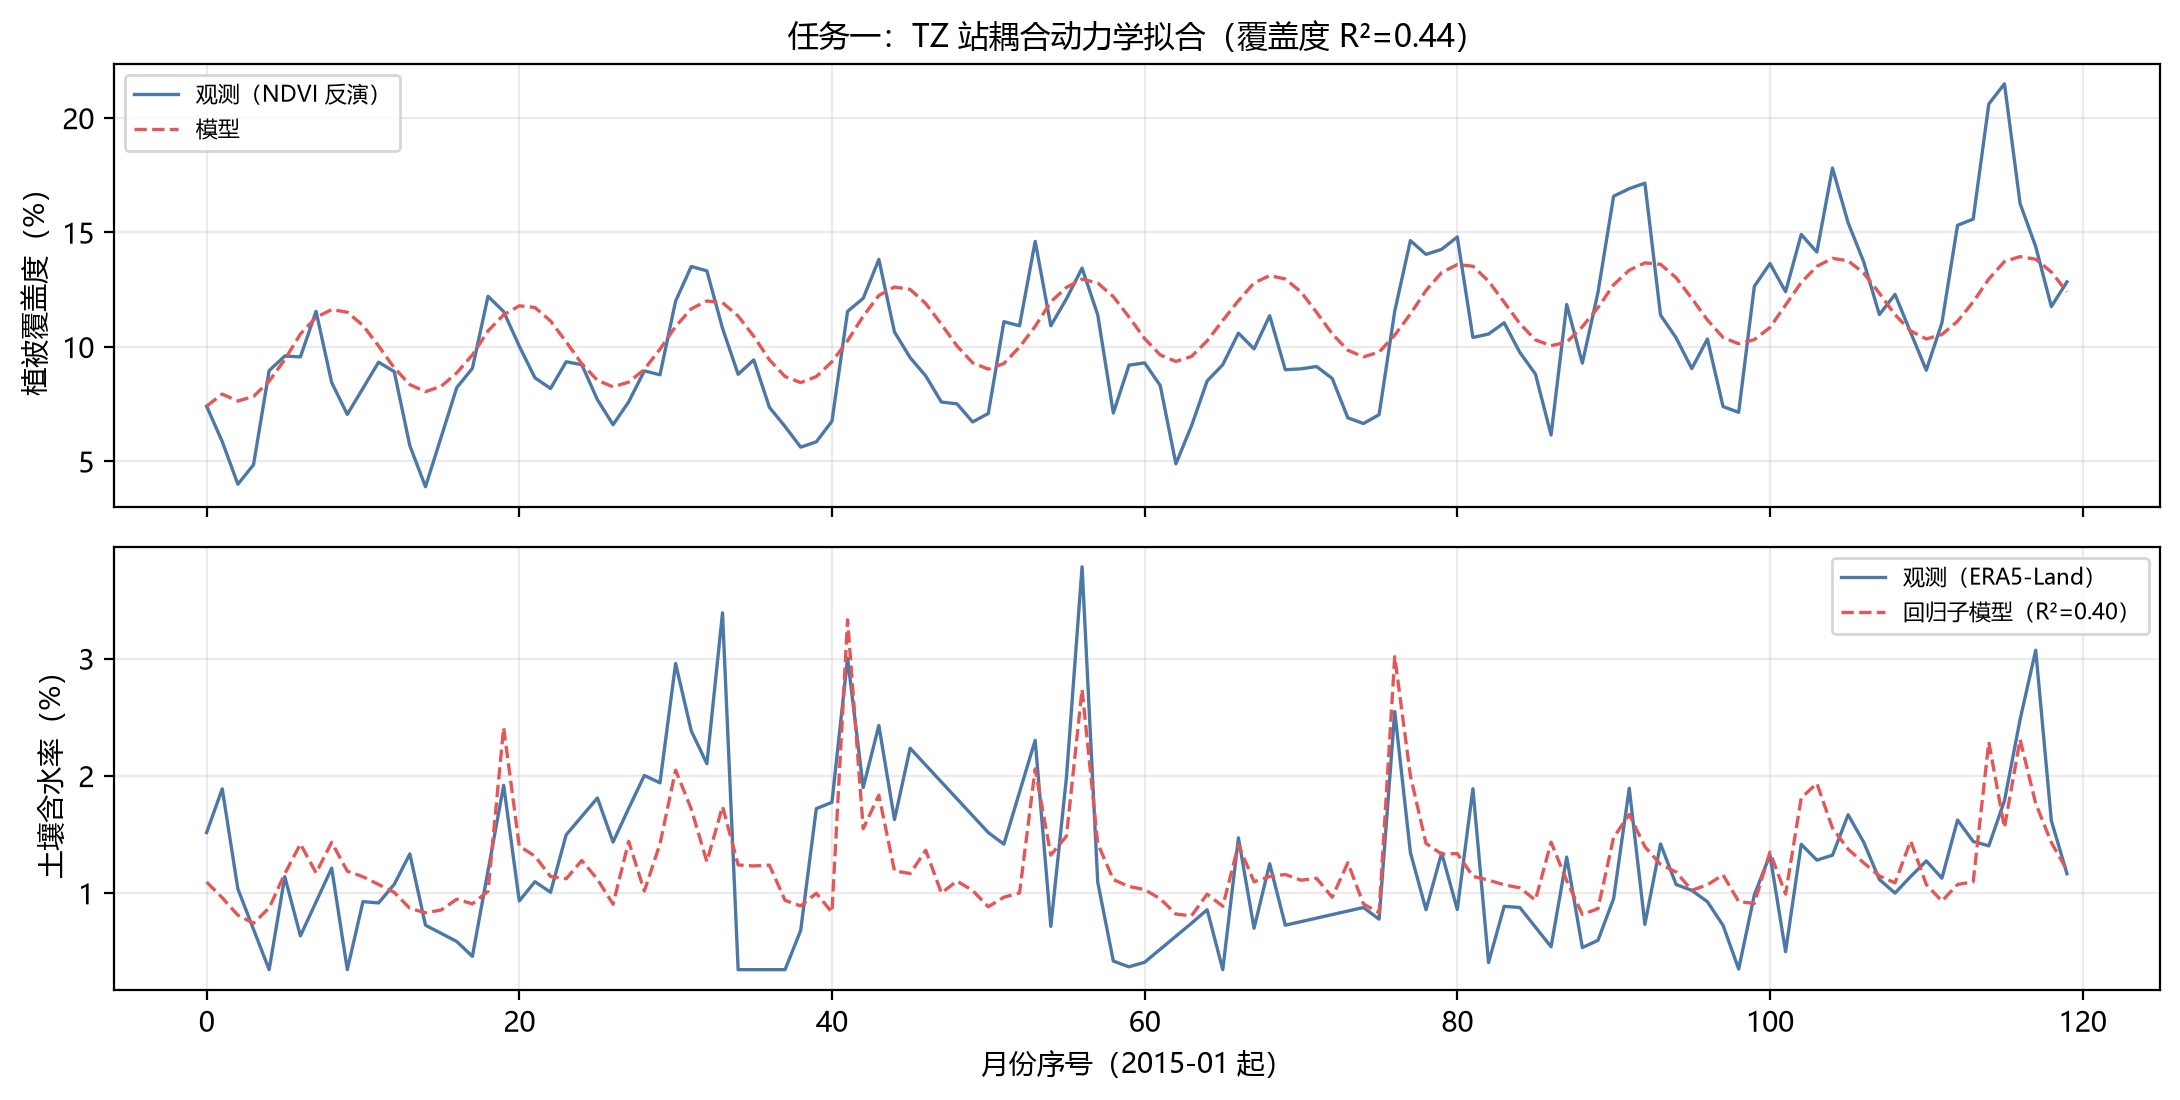
\includegraphics[width=0.90\textwidth]{figs/image1.png}
\end{figure}
图 1  ERA5-Land 与 NASA POWER 的逐月散点（虚线为 1:1 线）


\section*{七、数据的边界：哪些是观测、哪些是计算、哪些是情景}
表 7  数据集中各变量的性质界定


\begin{table}[H]\centering\small\setlength{\parskip}{2pt}
\begin{tabularx}{\textwidth}{|X|X|X|X|}
\toprule
\textbf{类别} & \textbf{变量} & \textbf{性质} & \textbf{说明} \\\\
\midrule
观测/再分析 & 风速、气温、降水、土壤含水率 & \textbf{真实数据} & ERA5-Land 同化产品，公开可复现 \\\\
遥感观测 & NDVI & \textbf{真实数据} & MODIS MOD13Q1 250 m 像元值 \\\\
派生量 & 植被覆盖度、输沙率、输沙势 & \textbf{由真实数据计算} & 公式已发表，仅输沙率含一个站级标定系数 \\\\
情景参数 & 累计治理面积、投资、补水量 & \textbf{非观测} & 属决策变量，由优化模型设定，不在数据集中冒充观测 \\\\
\bottomrule
\end{tabularx}
\end{table}
这一区分很重要：把“治理面积”当观测数据写进论文，等于凭空造一个国家的统计数字；把它明确定义为决策变量，反而是任务二建模的出发点。


\section*{八、复现步骤与更新方法}
表 8  复现流程


\begin{table}[H]\centering\small\setlength{\parskip}{2pt}
\begin{tabularx}{\textwidth}{|X|X|X|X|}
\toprule
\textbf{步骤} & \textbf{脚本} & \textbf{作用} & \textbf{耗时} \\\\
\midrule
1 & 01b\_fetch\_ndvi.py & 并发抓取 MODIS NDVI 分块并缓存 & 约 4 分钟 \\\\
2 & 01\_fetch\_real\_data.py & 抓取气象/土壤水 + 读取 NDVI 缓存 + 组装面板与派生量 & 约 5 分钟 \\\\
3 & 02\_crosscheck\_power.py & NASA POWER 交叉验证，出表与图 & 约 1 分钟 \\\\
4 & preprocess.py & 12 步清洗、插补、特征与划分 & 约 10 秒 \\\\
\bottomrule
\end{tabularx}
\end{table}
更新到 2025 年及以后：把 01b\_fetch\_ndvi.py 与 01\_fetch\_real\_data.py 顶部的 Y1 改为目标年份即可，脚本会自动按年切块抓取；缓存机制保证只下载新增年份。若接口格式变化，脚本的 http\_get 已有重试与错误提示。


\section*{九、数据集引用格式（GB/T 7714）}
[1] Zippenfenig P. Open-Meteo.com Weather API[DS/OL]. Zenodo, 2023. https://doi.org/10.5281/ZENODO.7970649.

[2] Hersbach H, Bell B, Berrisford P, et al. The ERA5 global reanalysis[J]. Quarterly Journal of the Royal Meteorological Society, 2020, 146(730): 1999-2049.

[3] Didan K. MOD13Q1 MODIS/Terra Vegetation Indices 16-Day L3 Global 250m SIN Grid V061[DS/OL]. NASA EOSDIS Land Processes DAAC, 2021. https://doi.org/10.5067/MODIS/MOD13Q1.061.

[4] Carlson T N, Ripley D A. On the relation between NDVI, fractional vegetation cover, and leaf area index[J]. Remote Sensing of Environment, 1997, 62(3): 241-252.

[5] Lettau K, Lettau H. Experimental and micrometeorological field studies of dune migration[M]//Exploring the World's Driest Climate. Madison: University of Wisconsin, 1978: 110-147.

[6] Fryberger S G. Dune forms and wind regime[M]//A Study of Global Sand Seas. Washington: USGS, 1979: 137-169.


\section*{十、已知局限与使用建议}
\textbf{ERA5-Land 的 9 km 格点 ≠ 站点观测}。沙漠腹地地表极不均匀，格点风速可能低估阵风峰值，导致输沙率偏低；建议在论文中用 NASA POWER 或台站数据做一次偏差订正，并在敏感性分析中讨论 $\pm$20\% 的影响。

\textbf{MODIS 250 m 存在混合像元}。绿洲边缘站点（库尔勒、尉犁、阿拉尔）的像元内混有农田与裸沙，$mathrmFVC$ 可能被高估；若条件允许，可用 Landsat 30 m 做局部校核。

\textbf{输沙率是估算值而非观测值}。公式系数 C 与阈值 u\_t 的不确定性会整体平移量级，所以它适合用来驱动“相对变化”与“分区对比”，不适合直接引用绝对吨数作为结论。

\textbf{冬季 NDVI 缺测集中在 11—2 月}。这段时期覆盖度本身很低（<10\%），插补误差对年际趋势影响有限，但对“春季起沙—植被恢复”的时序细节有影响，建议在图中标注缺测时段。


\end{document}
